\newpage
\section {Билет 9. IP, TCP, UDP, VPN, NAT}

\begin{center}
	\textit{\underline{Протокол IP}}
\end{center}

\href{https://ru.wikipedia.org/wiki/IP}{IP} - специальный протокол,позволяющий осуществлять передачу сообщений между устройствами, находящимися в одной сети посредством идентификации этих устройств 4-байтовыми кодами (адресами).

Его работу можно полностью сравнить с работой Почты России. Если положить письмо в ящик, то оно \textbf{может быть} дойдёт до адресата. При этом, если положить 10 писем в ящик, то какое-то количество из них, наверняка, дойдёт, однако \textbf{неизвестно, в каком порядке}.

Естественно, в таких условиях программам работать было бы не комфортно, поэтому на базе протокола IP были придуманы более хитрые протоколы, про которые мы и поговорим далее.

\begin{center}
	\textit{\underline{Протокол UDP}}
\end{center}

\href{https://ru.wikipedia.org/wiki/UDP}{UDP} - протокол на базе IP-протокола, позволяющий обмениваться данными. Работает следующим образом: данные разбиваются на пакеты, которые по своему размеру подходят для передачи по IP-протоколу, и отправляет эти пакеты, пронумеровав их. На стороне адресата эти пакеты посредством нумерации собираются обратно в исходные данные.

UDP \textbf{не поддерживает} подтверждение о получении пакета, то есть, что-то, возможно, не дойдёт. Однако внутри одного пакета данных UDP гарантирует, что все данные дойдут в целостности (если они вообще дойдут).

Используется в основном в стриминговых передачах (например, онлайн-трансляция видео или аудио, передача показаний датчиков в реальном времени). Основная идея - в отличие от TCP, неважно, если какие-то данные не дошли. Ну будет пробел и будет (не показывать же вам не дошедшие кадры из фильма через 5 секунд, как вы уже этот момент просмотрели).

\begin{center}
	\textit{\underline{Протокол TCP}}
\end{center}

\href{https://ru.wikipedia.org/wiki/Transmission_Control_Protocol}{TCP} - более сложный протокол передачи данных. Всё так же режет данные на более мелкие пакеты и нумерует их, однако отправка более хитрая.

TCP имеет буфер (для пример скажем, длины 4, хотя в реальности он гораздо больше), в котором размещены пакеты данных. Он отправляет данные из буфера и (в отличие от UDP!) ждёт.

Когда адресат получает, скажем, пакет данных №3, он посылает подтверждение, что третий пакет получен и контрольная сумма сошлась. После этого TCP убирает из буфера пакет №3 и помещает туда следующий (в нашем примере, пакет №5). По мере того, как приходят подтверждения, пакеты из буфера убираются и заменяются на новые.

Если на пакет долго не было подтверждения, то он отправляется ещё раз. Передача завершается только тогда, когда на все пакеты пришло подтверждение. Таким образом, можно гарантировать целостность передачи всего набора данных (или узнать, какие именно пакеты не дошли).

TPC используется, например, при передаче файлов или просто каких-то данных в реляционных системах.

\bigskip
При передаче данных возникает вопрос, насколько мелко стоит делить их на пакеты. Ведь при ошибке, скажем, 1 раз в 1000 байт, если делить данные на пакеты по 100 байт, ошибка будет в среднем в 1 из 10 пакетов (то есть, в среднем, повторно пересылать придётся около 10\% данных). А если делить на пакеты по 500 байт, то ошибка будет в каждом втором пакете.

С одной стороны, общий принцип пересылки - чем меньше пакет, тем больше вероятность, что он дойдёт. 

С другой стороны, в случае TCP-протокола, больше пакетов = больше ответных подтверждений, что будет забивать канал обратной связи. К тому же, не стоит забывать, что каждый пакет имеет заголовок (информация о том, кто отправитель, кто адресат, номер пакета, контрольная сумма и т.д.) фиксированного размера, не зависящего от разбиения. Поэтому, если размер заголовка, скажем, 100 байт, при разбиении данных на пакеты по 500 байт, итоговый размер пересланных данных вырастет на $\frac{1}{5}$. А если делить на пакеты по 100 байт, то итоговый размер пересылки вырастет в 2 раза.

\textbf{Мораль проста надо делить данные на как можно бОльшие пакеты.}

Одной отличительной чертой TCP является то, что он умеет адаптироваться к качеству сети. То есть, по мере пересылок данных TCP может просчитывать, как часто возникают ошибки в передаче, и варьировать оптимальный размер пакетов, на которые разбивает данные. Для этого он постепенно повышает размер пакетов, пока не дойдёт до \textit{критической секции}, когда повторные пересылки становятся непозволительно частыми из-за ошибок сети. Тогда он делает размер пакетов чуть поменьше, чтобы частота ошибок опять стала ''позволительной'', и держит эту \textit{оптимальную} планку.

Если в какой-то момент качество сети резко упало (например, гроза началась), то естественно, что оптимальный размер пакетов сразу станет не оптимальным и начнёт часто выдавать ошибки. В таком случае TCP делает несколько попыток передать данные такими пакетами, какие были, а после на основе статистики ошибок делает перерасчёт разбиения пакетов, чтоб опять всё стало оптимально. Когда качество сети поднимется, TCP опять начнёт постепенно увеличивать размер пакетов до оптимального.

Если сеть часто сбоит и работает нестабильно, можно самому поставить искусственную планку - \href{https://ru.wikipedia.org/wiki/Maximum_transmission_unit}{MTU}. Это параметр, определяющий максимальный размер пакета при разбиении набора данных. Больше него TCP не будет делать пакеты, даже если это было бы оптимальнее.

\begin{figure}[h]
	\centering
	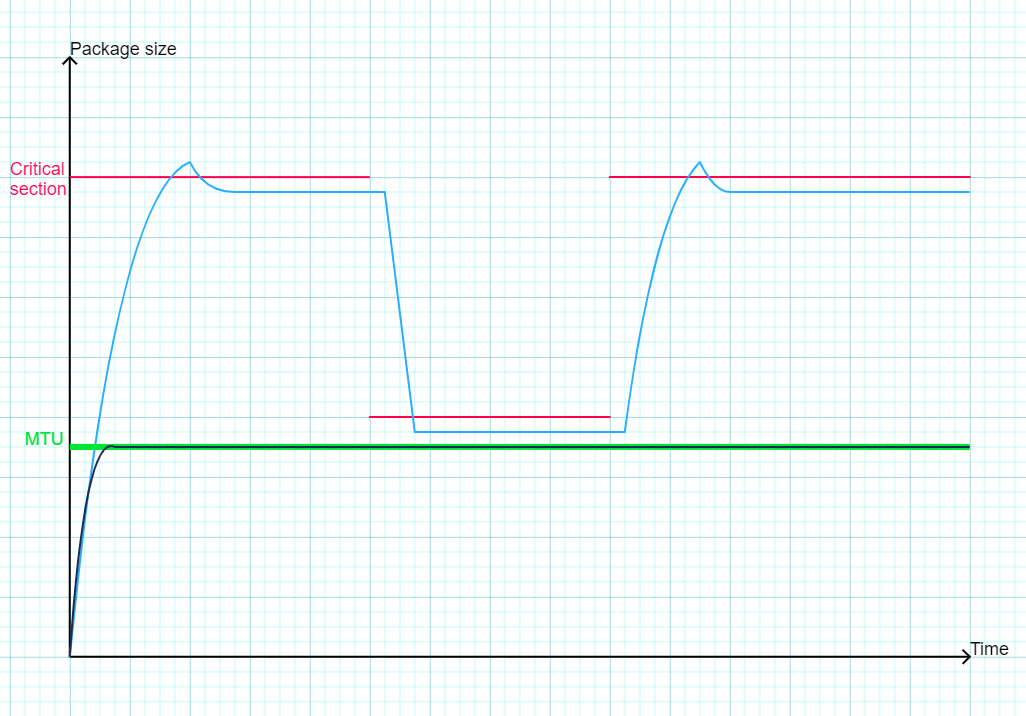
\includegraphics[scale=0.5]{9/09_01.png}
	\caption{Оптимизация TCP по размеру пакетов}
	\label{fig:graph_9}
\end{figure}

На рисунке~\ref{fig:graph_9} наглядно проиллюстрирован данный процесс. Красной линией отмечена \textit{критическая секция}, а голубой - график изменения размера пакетов данных по мере их передачи.

Пример работы при заданном параметре MTU (зелёная линия) отображён тёмно-синей кривой.

\textcolor{red}{\textbf{Внимание!}} Данный график является лишь схематической иллюстрацией и не претендует на точность.

\begin{center}
	\textit{\underline{Технологии NAT и VPN}}
\end{center}

Представим бытовую ситуацию: у нас дома есть WI-Fi роутер, подключённый к сети Интернет, и к этому роутеру в квартире подключены ПК, ноутбук, планшет, телефоны и ещё несколько устройств. С точки зрения внешней сети (Интернет) существует лишь роутер со своим IP-адресом. С точки зрения роутера, есть внешняя сеть + все устройства, которые находятся дома (у каждого из них есть свой локальный адрес, уникальный в этой локальной (домашней) сети). Тогда как нам отделять входящие и исходящие запросы, предназначаемые для ноутбука, ПК и прочих устройств по отдельности?

В решении этой задачи и заключается суть технологии \href{https://ru.wikipedia.org/wiki/NAT}{NAT}. Принимая пакет от локального компьютера, роутер смотрит на IP-адрес назначения. Если это локальный адрес, то пакет пересылается другому локальному компьютеру. Если нет, то пакет надо переслать наружу в интернет. Но ведь обратным адресом в пакете указан локальный адрес компьютера, который из интернета будет недоступен. Поэтому роутер «на лету» транслирует (подменяет) обратный IP-адрес пакета на свой внешний (видимый из интернета) IP-адрес и меняет номер порта (чтобы различать ответные пакеты, адресованные разным локальным компьютерам). Комбинацию, нужную для обратной подстановки, роутер сохраняет у себя во временной таблице. Через некоторое время после того, как клиент и сервер закончат обмениваться пакетами, роутер сотрёт у себя в таблице запись об n-м порте за сроком давности.

NAT меняет лишь заголовок и не трогает само ''тело'' передачи (посылает пакеты в таком виде, в каком их получил). Из-за этого сама по себе пересылка данных является незащищённой (то есть, если вы захотите переслать пароли с одного сервера на другой через Интернет, то потенциальный злоумышленник сможет их прочитать где-то по пути передачи).

\bigskip    
Для построения защищённых каналов связи используется \href{https://ru.wikipedia.org/wiki/VPN}{VPN}. Представим, что у нас есть два сервера, у каждого из которых какой-то свой закрытый контур (внутри которого уже используется, например, NAT), и мы хотим провести между ними соединение через Интернет. VPN помогает установить сетевое соединение поверх сети Интернет, создавая защищённый канал, проходя через который, данные будут шифроваться на входе и расшифровываться на выходе.
Таким образом, даже если потенциальный злоумышленник захочет прочитать эти данные (да, он всё ещё может где-то по пути пересылки данных увидеть их), то не сможет, ведь они зашифрованы. Недостатком VPN, очевидно, является скорость, ведь шифровать и расшифровывать данные - не самая быстрая операция.